\documentclass{template}
\usepackage{color}
\usepackage[hyphens]{url}
\usepackage{longtable}
\usepackage{graphicx}
\usepackage{enumitem}
\usepackage{pdfpages}
\usepackage{hyperref}

\def\etal{{\it et al.~}}
\newenvironment{packed_enum}{
\begin{enumerate}
  \setlength{\itemsep}{1pt}
  \setlength{\parskip}{0pt}
  \setlength{\parsep}{0pt}
}{\end{enumerate}}
\newenvironment{packed_item}{
\begin{itemize}
  \setlength{\itemsep}{1pt}
  \setlength{\parskip}{0pt}
  \setlength{\parsep}{0pt}
}{\end{itemize}}

\begin{document}

\title{Tor's Usability for Censorship Circumvention}
\numberofauthors{1}
\author{
 \alignauthor Linda N. Lee, David Fifield, Nathan Malkin \\
   \vspace{0.5em}
   \affaddr{University of California, Berkeley} \\
   \affaddr{\{lnl,fifield,nmalkin\}@cs.berkeley.edu}\\
}
\maketitle

\begin{abstract}
Tor has grown beyond its original purpose as an anonymity tool and has 
since become an important censorship circumvention tool. It is now listed
as one of the ways that normal people use Tor \cite{whotor}.
We specifically examine its usability as a censorship circumvention tool,
an essential facet for adoption and use.  
We focus our analysis on the connection configuration interface of Tor browser,
as censorship circumvention requires correct transport configurations.
We will conduct a large-scale user study examining 60-100 of users 
on how they navigate Tor's configuration wizard to complete seven browsing tasks 
in three different adversarial settings. Our study combines quantitative measurements (interface
paths taken to success, time to success, and which configuration was chosen) and
qualitative measurements (if users were comfortable with use, what was most confusing, and 
if they would use the browser again). The first phase of the study will evaluate if and how 
easily users can circumvent censorship using Tor Browser. The second phase
of the study will test improvements to the interface and an alternate interface. 
Our goal is to integrate positive usability changes into the Tor Browser. Since
the configuration interface is modular and does not require changes to the Tor Browser
functionality, these changes will be easy to deploy. 

\end{abstract}

\keywords{Censorship, Security, User Studies, Anonymity, Tor}

\section{Tor}
\noindent {\bfseries Usability}
Tor is primarily known as the most widely used anonymity tool today. 
For this reason, user studies on Tor have been solely about the usability of Tor as an
anonymity tool. Norcie~\cite{norcie2012eliminating} conducted an experiment which identified 
``stopping points'' in Tor browser,  documenting points when people would get frustrated enough 
to stop using Tor. To our knowledge, that has been the only published user study of Tor. 
Since then, Tor has had a lot of updates. There have been been no published usability evaluations of
Tor Browser since the introduction of the 4.0 series, which introduced radical UI changes. 
Lee and Fifield \cite {uxsprint} ran a small pilot study testing the download, install, and user interface of Tor Browser. 
This study uncovered a number of bugs and stopping points. Changes made are reflected in series 
5.1 and later. \\

\noindent {\bfseries Scoping}
There are still many features of Tor that are left unevaluated through user
research --- such as advanced web tasks (e.g., accessing hidden services), the
configuration menu to connect to the Tor network, configuring automatic
updates, and identity/cookie management. Rather than selecting the features to
study in isolation,
we decided to focus on an important use case of Tor browser: censorship circumvention. 
Internet censorship is pervasive across the world today \cite{faris2008measuring}, with 
some countries blocking censorship circumvention tools as well \cite{winter2012great}. 
To our knowledge, this is the first user study investigating the usability of Tor as a 
censorship circumvention tool.\\

\noindent {\bfseries Motivation}
Changing the configuration interface would not require changes to the 
Tor Browser functionality, making any suggested improvements very practical to 
deploy in a short period of time. {\color {red} Additionally, people are just literally
being censored everywhere so a lot of people are using it for this purpose. So 
we want this to be usable for that purpose.} 

\section{The Configuration Interface}

\noindent {\bfseries Overview}
The Tor Browser provides a configuration interface to guide users through setting up 
their connection to the
Tor network. While people in most countries can connect to Tor using the
dialog's default settings, citizens in certain censorship environments must
make use of additional settings, such as bridges, proxies, or both. 
{\color {red} definition of a bridge, definition of a proxy}   %%%
Our study  will explore how well this interface successfully guides users to 
correctly configuring their browser.\\

\begin{figure}[h]
\label{fig:bridges}
  \centering
    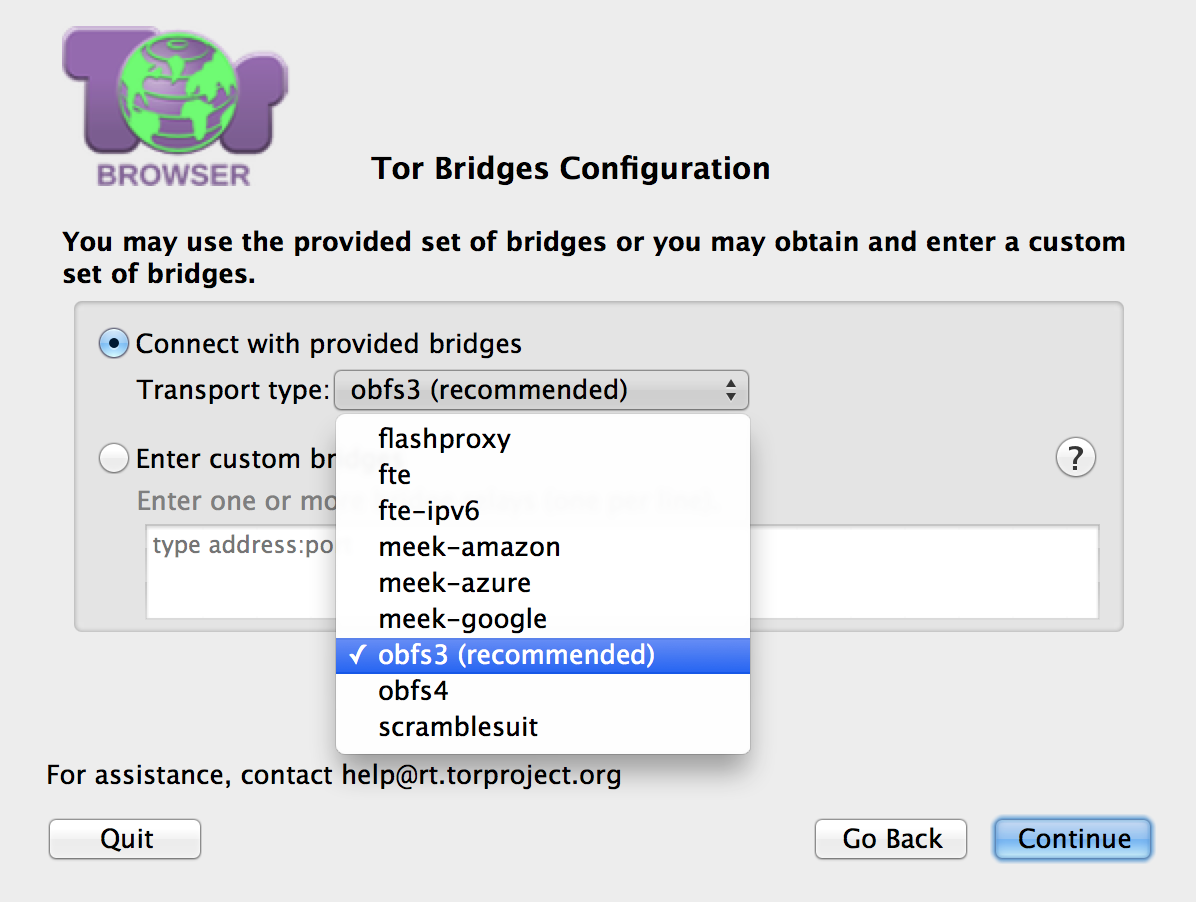
\includegraphics[width=0.5\textwidth]{configuration-screenshot.png}
    \caption{The Tor Bridges Configuration window of the Tor configuration
    interface. Tor users in censored environments and some of our participants
    will be required to select the correct bridge for circumventing censorship.
    Note that the interface prompts users to choose a transport type, which can be
    the source of confusion. Bridges are non-listed guard relays to the Tor
    network; transports, supported by bridges, obfuscate traffic in
    different ways.}
\end{figure}

\noindent {\bfseries Configuration Flow}
There are five general paths a user can take through the Tor Browser connection
configuration interface. {\color {red} These paths are shown in Figure ~\ref{fig:interface}}. 
The configuration interface asks a series of questions to 
the user to determine if the user requires a bridge or proxy when connecting to 
the Tor network. Depending on how the user answers these questions, a user 
has give paths through the configuration, as follows: 

\begin{itemize} \itemsep1pt \parskip0pt \parsep0pt
\item {\bfseries Path 1}:  Connect directly
\item {\bfseries Path 2}:  Yes bridge, no proxy, connect
\item {\bfseries Path 3}:  Yes bridge, yes proxy, connect 
\item {\bfseries Path 4}:  No bridge, yes proxy, connect 
\item {\bfseries Path 5}:  No bridge, no proxy, connect 
\end{itemize}
 
\begin{figure*}[t]
\label{fig:interface}
  \centering
    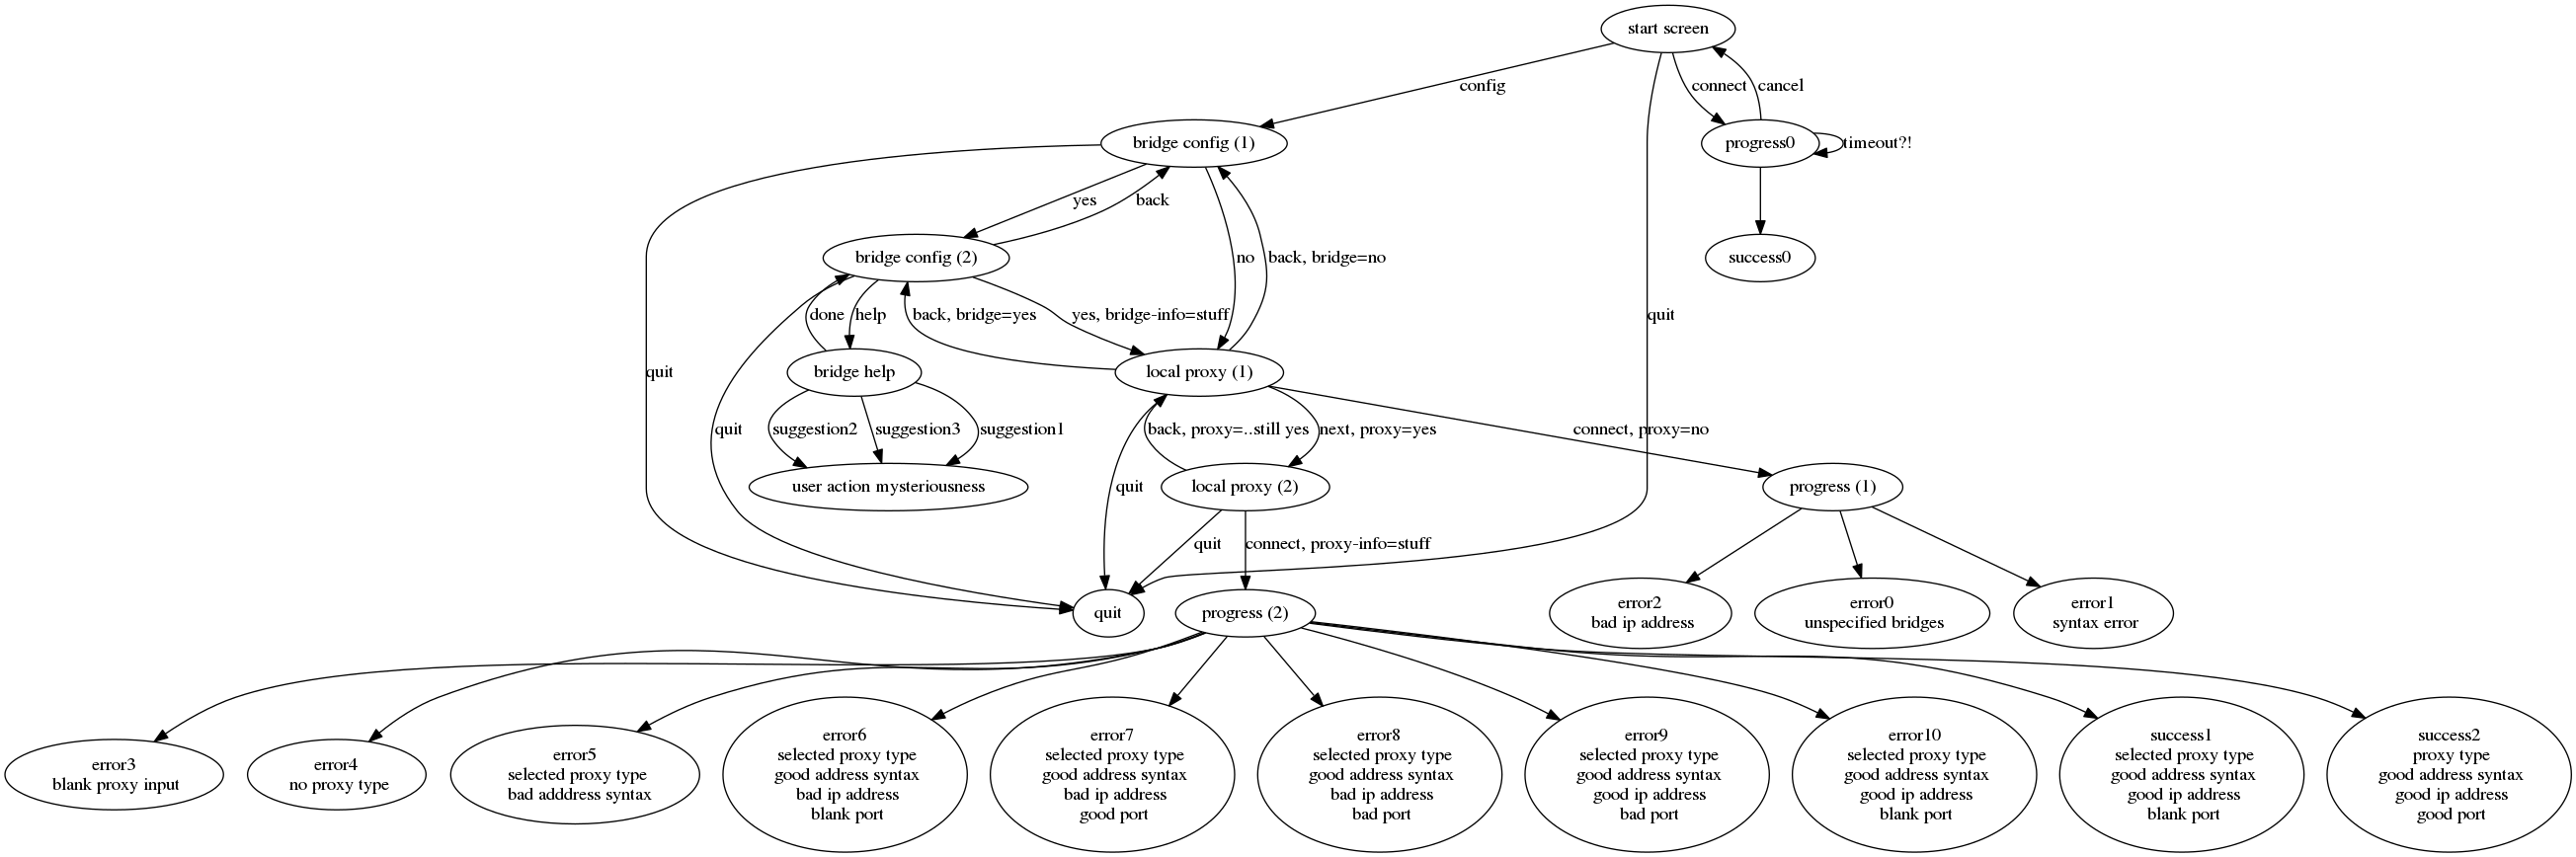
\includegraphics[width=\textwidth]{../torconfig.png}
    \caption{This flow chart shows all of the possible paths taken through the
    Tor configuration interface. A state represents a window in the interface,
    with the exception of the leaves, which indicate the final action taken by
    the interface (``q'' for quit, ``s'' for success, and ``e'' for error). The
    transitions between the states indicate which user action causes that
    transition. The cause for error is can be found
\href{https://github.com/lindanlee/circumvention-ux-tor/blob/master/torconfig.dot}{here}.}
\end{figure*}

Upon the startup of the configuration interface, a user is asked to describe their 
current situation. If their Internet connection is censored or proxied, the user 
clicks ``Configure'' to configure bridge and proxy settings. Otherwise, the user
clicks ``Connect'' to connect directly to the Tor network. 

If a user is not connecting directly to the Tor network, then they are asked to 
configure a bridge (as seen in {\color {red} TODO}, the title of the window during configuration %%%
is ``Tor Bridges Configuration''). We suspect that the reason for configuring a bridge
first before a proxy is that more people need to configure bridges than proxies,
but this is not known. The bridge configuration asks the users if their ISP blocks
or censors connections to the Tor Network. The assumption here is that users will 
not know if they need a bridge or not, but that they are equipped to answer if their
current network environment censors the Tor Network. The configuration interface 
uses this answer to deem if the user needs a bridge. A yes to this question would
require a bridge while a no to this question would not. If they answer yes, they are 
asked to configure the bridges. If they answer no, then the configuration interface 
moves on to configuring proxies. 

If a user who is not directly connecting to the Tor network is finished configuring
a bridge or has answered that they do not need a bridge, they are asked to 
configure a local proxy (as seen in {\color {red} TODO}, the title of the window during %%%
configuration is ``Local Proxy Configuration''). The proxy configuration asks the 
users if they need to use a local proxy to access the Internet. The assumption 
is that people will not know the answer to this question, so there is a text instructing
users how to find the answer to this question below the question. If the answer to
the question is yes, the user needs a proxy and is taken to a screen where they are
asked to configure the proxy settings. If the user does not need a proxy, then the 
configuration interface attempts to connect to the Tor network with all the 
given inputs up to this point so far. 

Note that a user can decide to click ``Configure'' because they believe the 
Internet connection is censored or proxied, but then answer the bridge and proxy
questions in such a way that they deemed that they do not need a bridge or proxy 
after all. In this case, clicking the ``Connect'' button after the above configuration steps
would be equivalent to clicking ``Connect'' on the first screen. \\ 


\noindent {\bfseries Things that are good about the interface} %% fix this so it's not so casual
{\color {red} 
Talking to users, ``this will work in most situations,'' help button, support email.
putting the bridge configuration before the proxy, etc.... \\
}

\noindent {\bfseries Things that could be improved about the interface }%% fix this so it's not so casual
{\color {red} 
clarify between bridges and proxy, getting rid of redundant text, etc.  \\
}

\noindent {\bfseries Hypotheses} We expect that the average user will
struggle to connect because they lack knowledge of the technical terms and
mechanisms required for circumvention (such as pluggable transports) and cannot
obtain information not explicitly provided by the user interface (e.g., IP
addresses of non-publicly listed bridges).

\begin{itemize} \itemsep1pt \parskip0pt \parsep0pt
\item  {\bfseries H1}: people don't know what a bridge or proxy is. > ask participants to define these terms in the survey.  
\item  {\bfseries H2}: people don't know what the difference between a bridge and a proxy is > ask if people can distinguish them. 
\item  {\bfseries H3}: people do not know when bridges or proxies are necessary > ask them this in the survey.  
\item  {\bfseries H4}: proxies cause confusion when configuring bridges. screen recording: see if people click on proxies (none of the environments require a proxy)
\item  {\bfseries H5}: people will favor familiar-sounding transports (i.e. meek-google versus meek-azure or scramblesuit) > see screen recordings, ask in survey for which transports were picked in which order and why they chose the final transport.  
\item {\bfseries H6}: (some dialogue is redundant. see opening window: "before you connect..." and bridge2 window: "you may use...") > we can try asking if people find these things useful, if they would prefer the interface without it, or if they read it.  
\end{itemize} 

\section{Methodology} 

We are going to aim for 5 users per censorship environment, improvement, 
and alternate interface. We are going to pre-screen our participants so that 
we have a good mix of gender, age, technical background, and familiarity 
with Tor. 

Some references to keep in mind when explaining: 
\href{why 5 users}{http://www.nngroup.com/articles/how-many-test-users/}
\href{screening}{http://www.userfocus.co.uk/articles/screeners.html}
\href{summative and usability mixed model}{http://www.usabilitybok.org/summative-usability-testing}

\section{Methodology}

\noindent {\bfseries Experiment Logistics} 
The IRB protocol to run this user study has been approved (2014-12-6995). 
We plan to recruit 35-50 users for the purpose of this study,
making it the largest user study of Tor to date.  This study will be conducted at the
Experimental Social Science Laboratory (Xlab)
at the University of California, Berkeley, which consists of 36 laptops,
separated by cubicle walls. We will use individual host firewalls to simulate
censorship environments and will record computer screens to capture 
user activity. The total length of the experiment, including briefing, completing the censorship 
circumvention tasks, exit survey, and debriefing, will be about an hour.
Participants will be compensated \$30 for their time, which covers
minimum wage for an hour and any transportation costs to the lab.  \\

\noindent {\bfseries Experiment Flow} 
We will conduct three separate experiments as part of this study:
the first set to test the current configuration
interface, a second set to test the improved interface, and a third set to test the 
alternate configuration interface. The experiment flow will be the same across all 
sets of experiments, but the configuration interface will be different across sets. 

The experiment begins with the participants being informed that they are in a
simulated censorship
environment, where some --- but not all --- websites are blocked. We will
instruct them to visit a non-blocked website and a blocked website on a
``standard'' browser (one that is not used for censorship circumvention, such
as Chrome, Safari, or Firefox) to illustrate the situation.
Then, the participants will find out the role they they will be playing in the study.
This role is that of a regular citizen who is trying to visit blocked websites
for non-critical leisurely purposes,
and for whom the chance of risk is minimal. This information is given
to achieve
consistency across participants: behaviors may change if the tasks were 
critical or if there were great risks associated with configuration mistakes. 

After explaining the situation and their role, we will explain what Tor is, and
how they can use it if necessary, and instruct them to complete a set of
tasks which will require visiting blocked websites. Ultimately, the
participants will need to configure their Tor Browser to circumvent the
simulated censorship environment. These tasks have a three-fold purpose of
providing participants with feedback (if they did not correctly configure their
browser, they cannot reach the website),  motivating the participants to
configure the browser correctly, and providing the researchers with an
indicator of successful censorship circumvention.
Participants' screens will be recorded to capture how they configure
their browser, and to provide additional evidence that they have completed the
tasks.

After users complete the browsing tasks, we will administer a survey that 1)
measures demographics, technical fluency, and
familiarity with Tor and 2) collects qualitative feedback from
participants about their browsing experience as a whole
and the configuration interface specifically.
A rough draft of the survey can be
found
\href{http://www.surveygizmo.com/collab/2085559/Tor-Usability-Survey}{here}.

The experiment will conclude with a debriefing, which will inform that the
participants of their screen capture and obtaining re-consent for the
information. \\

\noindent {\bfseries Censorship Environment Simulation} 
We plan to simulate three censorship environments.
They are informed by our experience with pluggable transports
and knowledge of commonly seen censorship techniques.
They are not meant to perfectly replicate the network environment
in any particular country. Although inspired by reality, these
abstract simulations are intended to require distinct configurations
of the Tor Browser from our participants. \\

\begin{itemize} \itemsep1pt \parskip0pt \parsep0pt
\item {\bfseries Mild censorship} 
(Reflective of countries such as France and Australia.)
Certain domains are blocked. Reaching these 
domains requires a censorship circumvention 
tool. The default option to ``connect'' to the Tor network 
directly will circumvent this censor. Additional correct
bridge or proxy configurations are optional. 
\item {\bfseries Intermediate censorship} 
(Reflective of countries such as Tunsia.)
Certain domains are blocked. Censorship circumvention
tools are blocked. Since Tor is blocked by blocking all public Tor
relay nodes, the default option to ``connect'' to the Tor network
directly will fail. Any choice of a hard-coded bridge (see Figure ~\ref{fig:bridges})
or a valid non-public bridge will circumvent this censor.  
Additional correct proxy configuration is optional.
\item {\bfseries Comprehensive censorship} 
(Reflective of countries such as China and Syria.)
Certain domains are blocked. Censorship circumvention tools
are thoroughly blocked. Tor is blocked by blocking all public
Tor relay nodes, and the censor has examined source code to block
all hard-coded bridge relays in the configuration interface. The default option
to ``connect'' to the Tor network directly will fail. Choosing any bridges other than
``meek-amazon,'' ``meek-azure,'' and ``meek-google,'' will fail. This is because 
domain-fronting requires censors to block entire CDNs to also block this
transport (which will cause huge collateral blocking damage), making it resistant to agressive censorship environments.
(See ~\cite{fifield2015blocking} for additional details.)\\
\end{itemize}

\noindent {\bfseries List of Tasks} 
In our experimental setup, successful completion of 
these given tasks requires of correct configuration.
The difficulty of circumventing  censorship to visit the 
websites required for the tasks will vary depending on the 
simulated censorship environment. Since all participants will be given the 
same set of tasks, regardless of the censorship environment, 
the difficulty of completing the tasks remains constant assuming
correct configuration. The tasks themselves are not intended to
be challenging.

The tasks were inspired by the top Alexa sites,
an indication of representative and relevant browsing behavior. 
From these, we selected sites which were commonly censored, 
but filtered tasks that would require a participant to reveal private information 
(such as login information) for ethical considerations. These tasks
were further refined after performing a pilot study of the experiment. 
We hope the tasks convey an example of how of a user might 
browse the Internet in a censored environment. 

\begin{itemize} \itemsep1pt \parskip0pt \parsep0pt
\item Google search for the population of Zimbabwe. 
\item On YouTube, find a video playing Bach's ``Ode to Joy.''
\item Find the Amazon best-sellers in ``Movies \& TV.''
\item On Yahoo, find the exchange rate of dollars to euros.
\item Find the Wikipedia ``History'' portal's featured article. 
\item On Twitter, find the currently trending topics.
\item On Bing Maps, find directions from Times Square to Carnegie Hall.\\
\end{itemize}

\noindent {\bfseries Improved and Alternative Interfaces} We have yet to design the 
improvements to the interface, as they will be based on the data collected from 
the user studies on the current configuration interface. In general, we will measure the 
time it took to configure correctly, and help users avoid common mistakes. An alternate 
interface to automate the configuration process for the user has been proposed in the 
community. One concern about it is that the automation makes the connection process less transparent, 
and since there are countries who log Internet activity, automated attempts to obviously
use the Tor network could have the potential to be incriminating.\\

\noindent {\bfseries Exit Survey}
{\color {red} talk about the survey here.} 

\section{Results}

Problems: 

\begin{itemize} \itemsep1pt \parskip0pt \parsep0pt
\item {\bfseries Problem1:} People don't know how to choose between ``connect directly'' versus ``configure'' on the first screen. 
\item {\bfseries Problem 2:} People feel compelled to set up a bridge, even if they don't need one, because they do not know how censorship works. 
\item {\bfseries Problem 3:} When their first attempt to connect fails, people tend to first try changing the proxy settings, because that is the window visible after a failure (an artifact of the fact that it is the last window visible before the failure). 
\item {\bfseries Problem 4:} When the first attempt to connect fails, people don't know what to do or what to try next. 
\end{itemize}

Proof of problems: 

\begin{itemize} \itemsep1pt \parskip0pt \parsep0pt
\item {\bfseries Proof 1:} TODO
\item {\bfseries Proof 2:} TODO
\item {\bfseries Proof 3:} TODO
\item {\bfseries Proof 4:} TODO
\end{itemize}

Source of Problems: 

\begin{itemize} \itemsep1pt \parskip0pt \parsep0pt
\item {\bfseries Source 1: Users lack a mental model of how censorship works.} For instance, our participants did not know the difference between a bridge and a proxy or a censored website versus censored Tor relays. We suspect that this is the result of an accurate mental model of how the Internet works.  It would be unreasonable to assume that users should know this information, but some of this may be required to make a correct decision in the current interface. 
\item {\bfseries Source 2: The interface flow does not guide users down the ideal path.} Much of the real estate on bridge configuration is used for the ``custom bridges'' option, which is an option rarely used. The interface instructs users to check out Internet settings to see if they would require a proxy, but it turns out that people are not skilled at doing so. Because the interface redirects users to the proxy screen after failing to make a connection, most of our participants tried configuring a proxy after a connection had failed due to an assumption that the proxy was the reason for the failure. In reality, there was no proxy setup required for any simulated censorship environment in our experiment and participants should have configured a bridge. 
\item {\bfseries Source 3: There is little constructive feedback during failure cases.} When a connection seems to not work, our participants were unsure of if they should wait more or if they should try the connection with the same configuration again, both of which are viable strategies, depending on the situation. Although there are certain error messages which were helpful, most of the error messages were technical and not understood by our participants (Figure \ref{fig:error}). The interface does not give clear directions on what participants should do next if a connection fails. 
\end{itemize}

\begin{figure*}[t]
\label{fig:error}
  \centering
    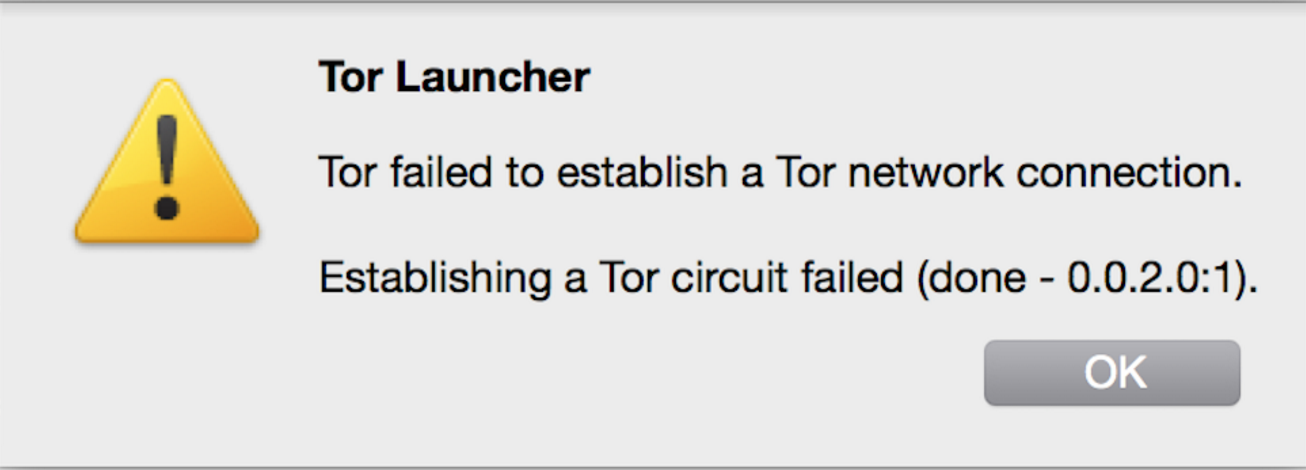
\includegraphics[width=\textwidth]{error.png}
    \caption{An example of a technical error message which our participants did not understand.}
\end{figure*}

\section{Design}

\section{Future Work}

We plan to finish the user study by the end of the semester. 
From this experiment, we hope to accomplish the following: 

\begin{itemize} \itemsep1pt \parskip0pt \parsep0pt 
\item {\bfseries Test an improved configuration interface} With the measurements collected
from testing the interface as-is, we will design and test improvements to minimize
time taken, paths taken, and error states reached.
\item {\bfseries Push changes} We have the support of Tor developers
to improve this interface. Additionally, since the configuration interface does not require 
any changes to the Tor Browser functionality, improvements to the interface will
be easy to deploy. 
\end{itemize}


\section{Discussion}

\section{Resources}
\noindent Our online artifacts of the work done during this class, Fall 2015,
are below: 
\begin{itemize} \itemsep1pt \parskip0pt \parsep0pt
\item \href{https://github.com/lindanlee/circumvention-ux-tor}{github repo with experiment plans, code, and paper}
\item \href {https://github.com/lindanlee/circumvention-ux-tor/blob/master/pilot/1-strict.mp4}{pilot video 1}
	\href{https://github.com/lindanlee/circumvention-ux-tor/blob/master/pilot/2-lax.mp4}{pilot video 2}
\item \href{https://github.com/lindanlee/circumvention-ux-tor/blob/master/setup/setup-environment}{experimental setup code: firewall and screen capture} 
\item \href{https://github.com/lindanlee/circumvention-ux-tor/blob/master/setup/takedown-environment}{experimental takedown code: saving files and cleanup} 
\end{itemize}

% from anonymity study
%Our online artifacts of study of Tor as an anonymity tool, such as 
%the summary, results, and resulting browser changes are below:
%\begin{itemize} \itemsep1pt \parskip0pt \parsep0pt
%\item \href{https://trac.torproject.org/projects/tor/wiki/org/meetings/2015UXsprint}{blog post summary}
%\item \href{https://blog.torproject.org/blog/ux-sprint-2015-wrapup}{changes made to Tor}
%\item \href{https://people.torproject.org/~dcf/uxsprint2015/}{subtitled screen videos}
%\end{itemize}

\bibliographystyle{abbrv}
\bibliography{circumvention-experiment.bib} 

\appendix
\section*{A1: Configuration Interface Windows}

\begin{figure}[h]
\label{fig:window1}
  \centering
    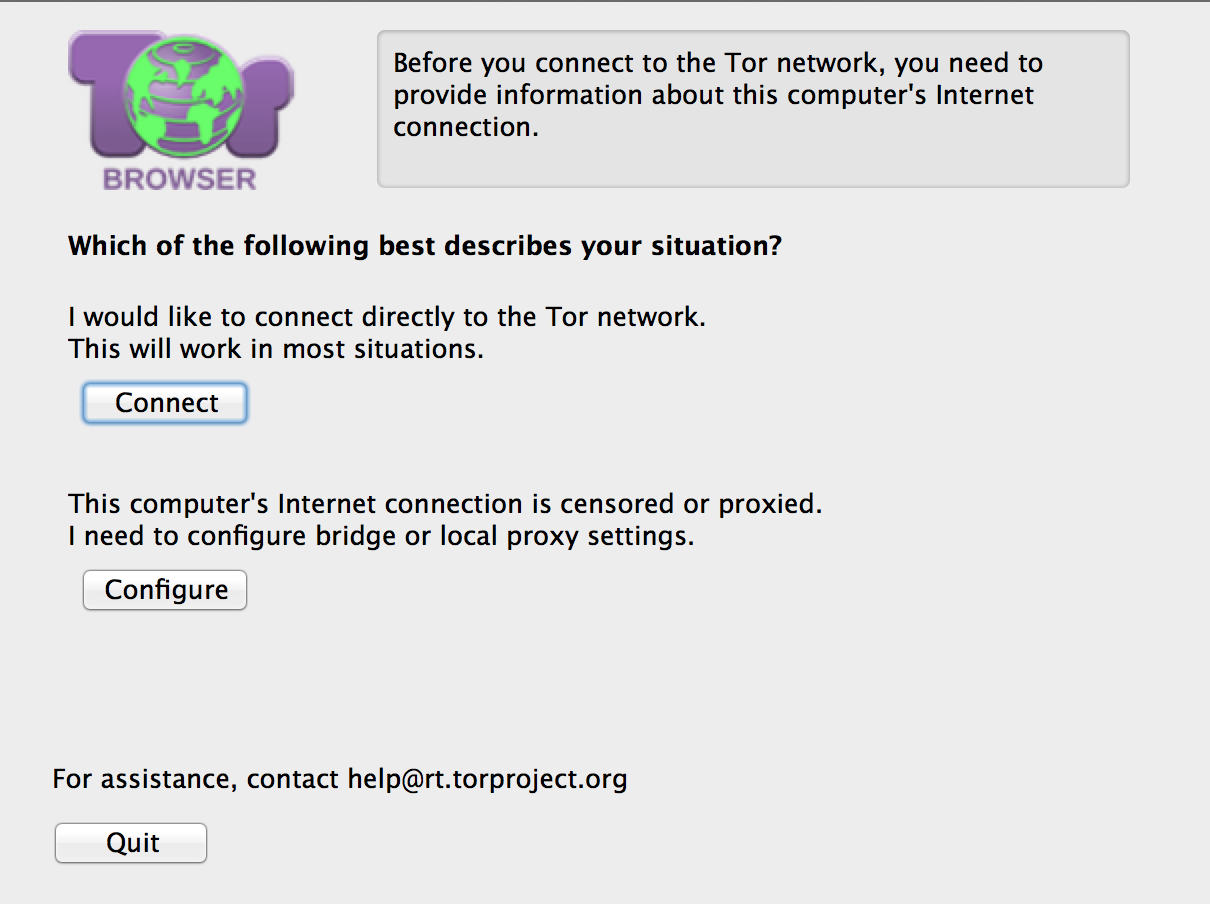
\includegraphics[width=0.5\textwidth]{window1.png}
    \caption{Window 1: the first configuration window shown to the user upon
    starting Tor Browser for the first time. Note that the interface's default choice
    is to connect directly through Tor. The interface also gives additional guidance
    to help users answer this question.}
\end{figure}

\begin{figure}[h]
\label{fig:window2}
  \centering
    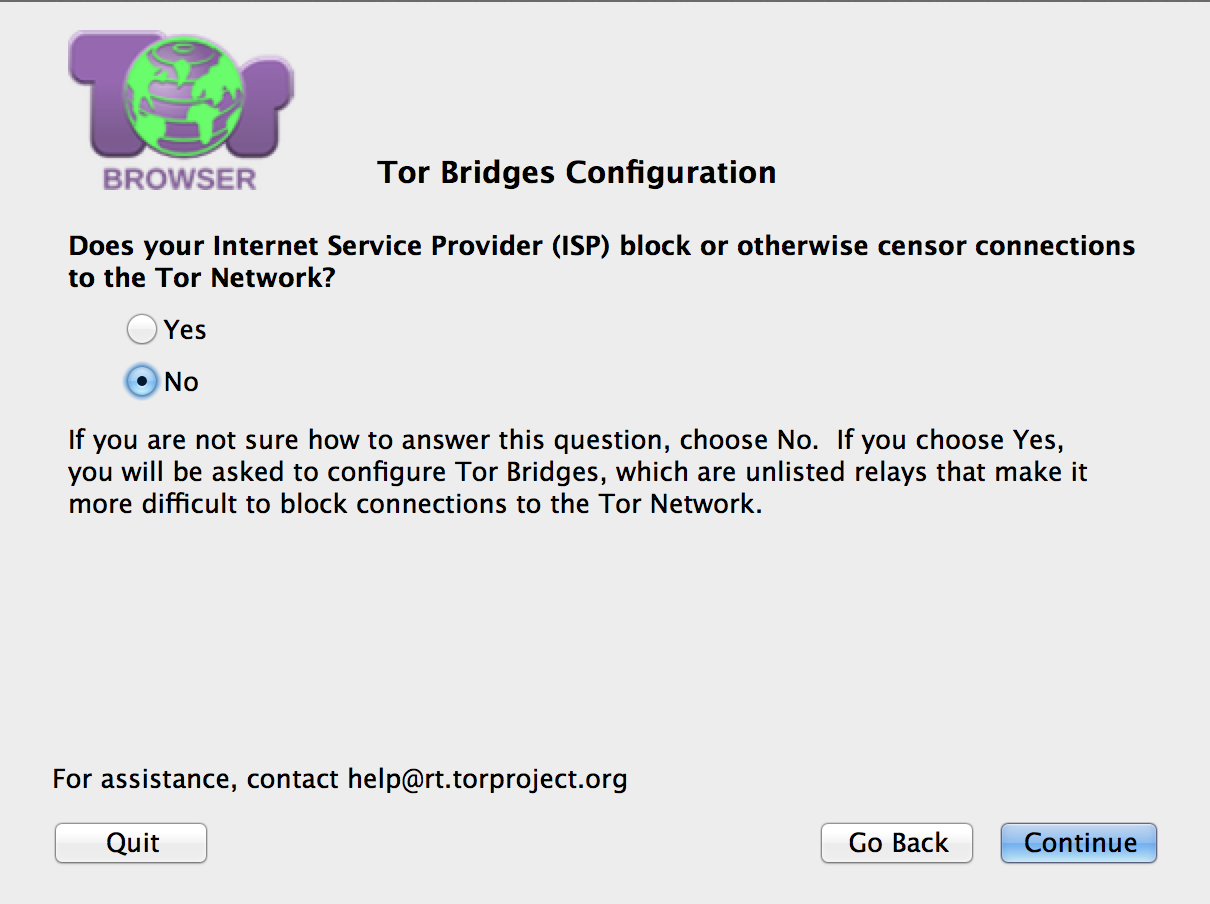
\includegraphics[width=0.5\textwidth]{window2.png}
    \caption{Window 2: This is the next window shown if a user chooses to configure 
    bridges or proxies. Note that the interface's default answer is ``No,'' 
    and also advises users to click ``No'' if they are unsure. The user can navigate to the 
    previous window by clicking ``Go Back,'' and continue configuration by clicking 
    ``Continue.''}
\end{figure}

\begin{figure}[h]
\label{fig:window3}
  \centering
    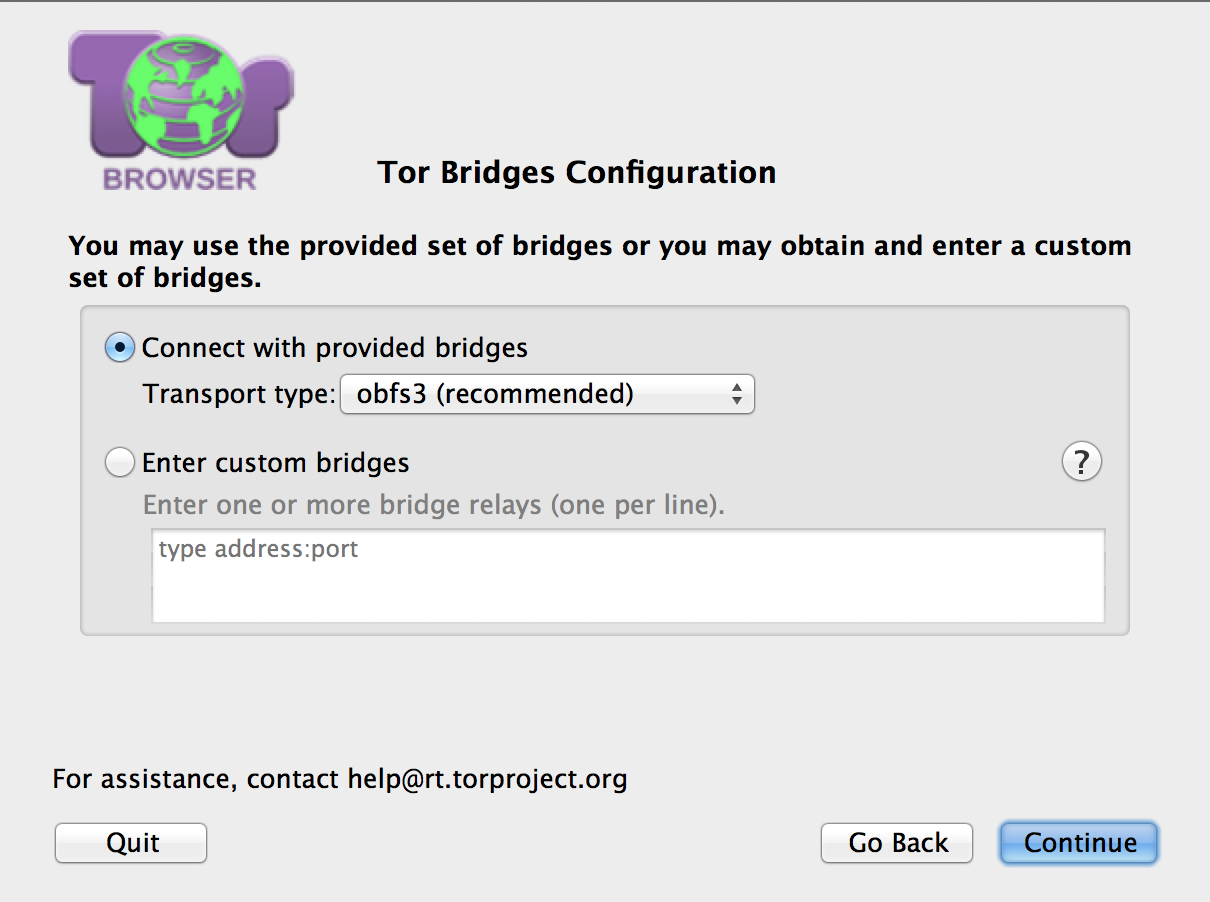
\includegraphics[width=0.5\textwidth]{window3.png}
    \caption{Window 3: This is the window shown when a user answers that a bridge 
    is required for the connection. Note that the default answer is to connect with a hard-
    coded bridge rather than to enter in a custom bridge, and to use the recommended 
    transport (obfs3). A possible source of confusion is that that the user is asked to choose 
    a transport type, when the interface clearly is asking for bridge configuration. The user 
    can navigate to the previous window by clicking ``Go Back,'' and continue configuration 
    by clicking  ``Continue.''}
\end{figure}

\begin{figure}[h]
\label{fig:window4}
  \centering
    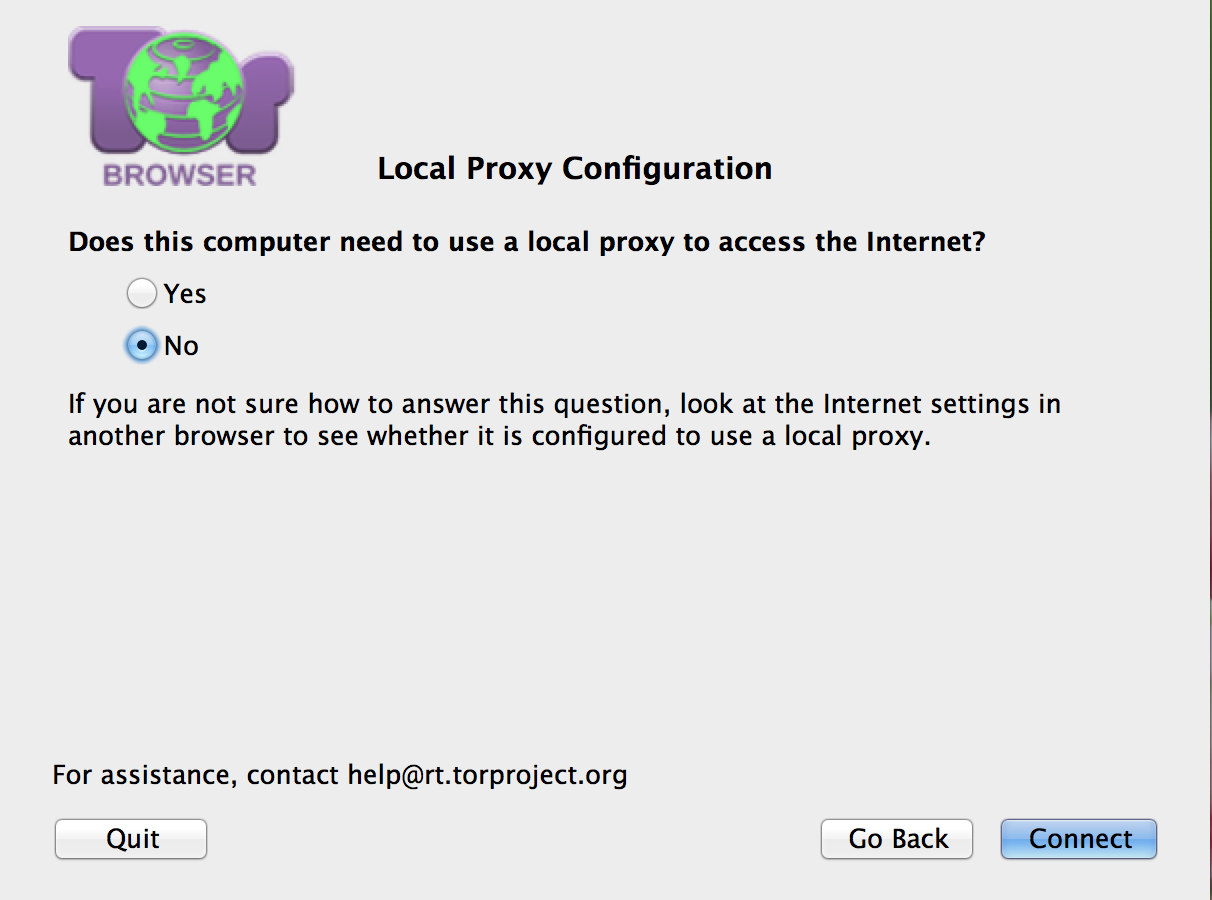
\includegraphics[width=0.5\textwidth]{window4.png}
    \caption{Window 4: This is the window shown after a user has deemed that a bridge
    is not required for the connection, or when the bridge configuration settings have been 
    chosen. Note that the default answer to if the user requires a proxy is ``No.'' Additionally,
    there is text to guide the users on how to answer this question. The user 
    can navigate to the previous window by clicking ``Go Back,'' and continue configuration 
    by clicking  ``Continue.''}
\end{figure}

\begin{figure}[h]
\label{fig:window5}
  \centering
    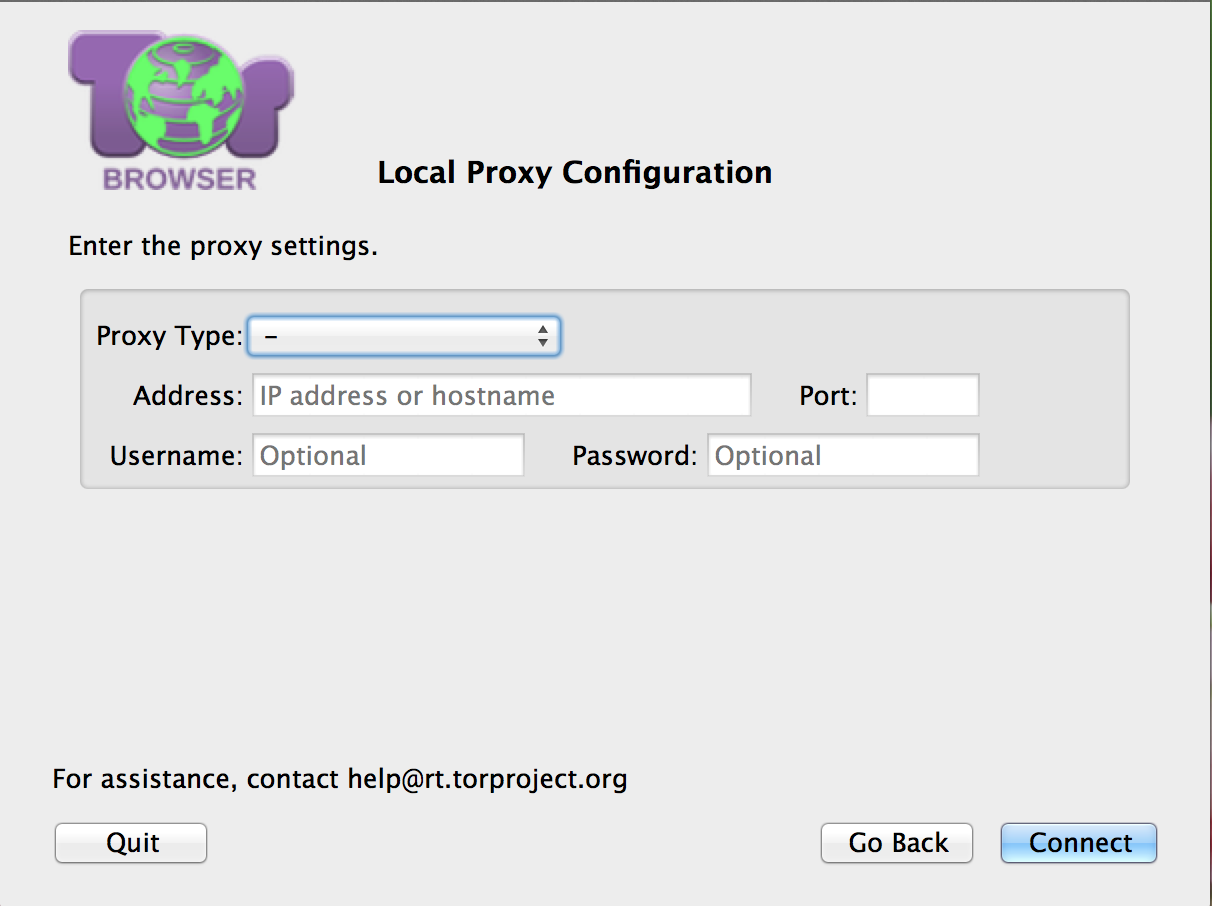
\includegraphics[width=0.5\textwidth]{window5.png}
    \caption{Window 5: This is the window shown when a user answers that a proxy is 
    required for the connection. Note that there are no default values in the answers, 
    where there were for bridges. Additionally, since this is the last window in the configuration
    interface, the options to navigate to other windows are to simply ``go back,'' or to 
    connect to the Tor Network.}
\end{figure}
\end{document}
